\chapter{Resultados Preliminares}
\label{ch:03-results}

% “Language, never forget, is more fashion than science, and matters of usage, spelling and pronunciation tend to wander around like hemlines.” 
% ― Bill Bryson, The Mother Tongue: English and How It Got That Way

Neste capítulo serão discutidos os resultados de múltiplos experimentos realizados a partir de diferentes tipos de modelagem de redes neurais. A primeira delas, baseada na pesquisa de Rumelhart e McClelland e discutida na Seção \ref{sec:arqFDD}.
A segunda, o modelo de Encoder-Decoder discutido na seção \ref{sec:enc-dec}. Para cada um destes experimentos, subdividem-se seus respectivos corpus entre treino (80\%) e validação (20\%). Essa partição tem como objetivo direcionar o modelo para um melhor desempenho diante de dados novos. Resultados de predições sobre alguns verbos da base de teste são exibidos no Apêndice. 

\section{Rede FFD}
\label{sec:ffd}

A rede desenvolvida possui uma camada de Input e uma de Output, ambas compostas por 460 unidades, cada unidade representando um Wickelfeature.

\subsection{Corpus}
\label{sec:corpus-ffd}

O corpus utilizado para o treinamento dessa rede foi baseado nas informações contidas nos sites \url{https://www.conjugacao.com.br/verbos-irregulares/} e \url{https://www.conjugacao.com.br/verbos-irregulares/}.\\

Primeiramente, foi realizada uma etapa de extração dos verbos e suas respectivas conjugações para um banco de dados local via técnica de \textit{webscraping}. Em seguida, os verbos irregulares foram selecionados manualmente para diferentes famílias. Alguns dos verbos irregulares apontados pela fonte não eram irregulares na conjugação específica de interesse e portanto foram realocados para o grupo de verbos regulares. Em seguida, os verbos foram transcritos manualmente para uma forma pseudo-fonética como demonstrada pela tabela \ref{tab:Tab1}. Dos 423 verbos extraídos, 20 foram considerados verbos sem possível agrupamento (verbos como "ir", "trazer" e "saber"), totalizando uma base de 214 verbos regulares e 209 regulares (50.59\% e 49.40\% respectivamente). A base foi em seguida segmentada entre treino (80\%) e teste (20\%) respeitando-se as proporções intra-classe.  

%colocar as tabelas de treino e teste
\subsection{Hiperparâmetros}

\begin{table}[H]
\centering
\begin{tabular}{ll}
Loss: & mean squared error \\
Optimizer: & adam \\
Activation: & softmax \\
Epochs: & 400 \\
\end{tabular}
\caption{Tabela Resumo Estrutural do Modelo FFD}
\label{tab:res1}
\end{table}

\subsection{Resultados}

O modelo FFD foi treinado em diferentes bases com diferentes arranjos proporcionais de verbos irregulares contra regulares. Esses testes foram realizados com o intuito de testar se a frequência de verbos irregulares pode influenciar no processo de aprendizado dos mesmos. Todos os modelos foram testados em 21 verbos, sendo 16 destes irregulares. A base de teste foi escolhida de modo a testar o modelo em famílias irregulares diversas. A Tabela \ref{tab:resultadosfdd} resume os resultados obtidos a serem discutidos na Seção \ref{sec:disc}.

\begin{table}[H]
\centering
\begin{tabular}{llllll}
 & \textbf{55\%} & \textbf{65\%} & \textbf{75\%} & \textbf{85\%} & \textbf{95\%} \\ \hline
\textbf{Acurácia} & 47.62\% & 38.10\% & 38.10\% & 42.86\% & 47.62\% \\
\textbf{Loss} & 1.92\% & 1.87\% & 1.57\% & 1.42\% & 1.22\%
\end{tabular}
\caption{Resultados para diferentes proporções de verbos irregulares na base de treino para a rede FDD.}
\label{tab:resultadosfdd}
\end{table}

\section{Encoder-Decoder}
\label{sec:seq2seq}

Como discutido na Seção \ref{sec:enc-dec}, os modelos do tipo Encoder-Decoder parecem promissores para o alcance dos objetivos propostos. Nessa seção são discutidos e comparados alguns testes que exibem a mesma arquitetura (Fig. \ref{fig:encdec}), porém alteram-se alguns dos hiperparâmetros possíveis e testam-se também bases de diferentes comprimentos.

A camada de Input do Encoder é inicializada a partir do tamanho do vocabulário. Nesse caso, considera-se vocabulário o número de caracteres únicos contidos na base de treinamento para a forma infinitiva dos verbos. Na camada de Input do Decoder, equivalentemente, o vocabulário da forma verbal conjugada.
%incluir ref Keras

Os outputs da rede Encoder são descartados e seus estados finais inicializam os pesos da rede Decoder. Por último, os outputs da rede Decoder passam por uma camada densa (sem recorrência).

%talvez acrescentar aqui que alguma referencia disse que mais camadas é bom pro aprendizado

\begin{figure}[H]
  \centering
  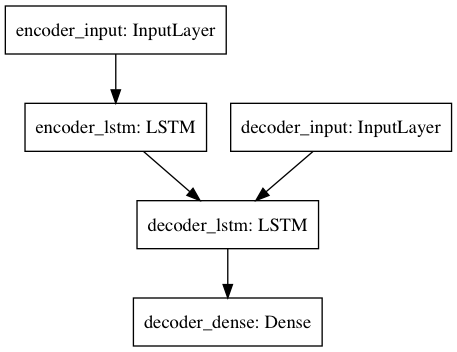
\includegraphics[width=0.5\linewidth]{img/draw-model6.png}
  \caption{Arquitetura Encoder-Decoder Desenvolvida}
  \label{fig:encdec}
\end{figure}

%ref[].

\subsection{Modelo Encoder-Decoder 1} 

\subsubsection{Corpus}
O modelo \textbf{Encoder-Decoder 1} foi treinado na base apresentada na Seção \ref{sec:corpus-ffd}, porém sem qualquer balanceamento relativo às proporções de verbos irregulares.

\subsubsection{Hiperparâmetros} 

\begin{table}[H]
\centering
\begin{tabular}{ll}
Numero de Amostras Treinamento: & 325 \\
Numero de Amostras Teste: & 100 \\
Numero de tokens unicos do Input: & 22 \\
Numero de tokens unicos do Output: & 26 \\
Comprimento maximo da sequencia para inputs: & 11 \\
Comprimento maximo da sequencia para outputs: & 13 \\
Loss: & categorical\_crossentropy \\
Optimizer & rmsprop \\
Activation & softmax \\
Epochs & 130 \\
Batch Size & 64
\end{tabular}
\caption{Tabela Resumo Estrutural do Modelo Encoder-Decoder 1}
\label{tab:res1}
\end{table}

\subsubsection{Resultados}

\begin{figure}[H]
  \centering
  \begin{subfigure}[b]{0.45\linewidth}
    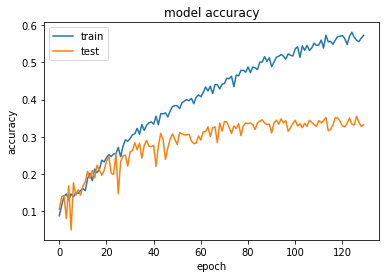
\includegraphics[width=\linewidth]{img/enc-dec-1.png}
    \caption{Resultados de Acurácia por Época}
  \end{subfigure}
  \begin{subfigure}[b]{0.45\linewidth}
    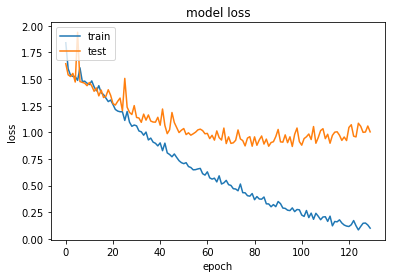
\includegraphics[width=\linewidth]{img/enc-dec-1-loss.png}
    \caption{Resultados de Custo por Época}
  \end{subfigure}
  \caption{Gráficos dos Resultados do Modelo}
  \label{fig:plots1}
\end{figure}

\begin{table}[H]
\centering
\begin{tabular}{llllll}
\textbf{Best Epoch Score} & \textbf{Val\_Acc} & \textbf{Vall\_Loss} & \textbf{Loss} & \textbf{Acc} & \textbf{Time} \\
97 & 0.342 & 0.867 & 0.290 & 0.508 & 2 min
\end{tabular}
\caption{Scores do Modelo Encoder-Decoder 1}
\label{tab:res-enc-dec-1}
\end{table}

\subsection{Modelo Encoder-Decoder 2}

\subsubsection{Corpus}
O modelo \textbf{Encoder-Decoder 2} foi treinado na base apresentada na Seção \ref{sec:corpus-ffd}, para o caso de proporção de 55\% de verbos irregulares. 

\subsubsection{Hiperparâmetros} 

\begin{table}[H]
\centering
\begin{tabular}{ll}
Numero de Amostras Treinamento: & 452 \\
Numero de Amostras Teste: & 21 \\
Numero de tokens unicos do Input: & 23 \\
Numero de tokens unicos do Output: & 27 \\
Comprimento maximo da sequencia para inputs: & 13 \\
Comprimento maximo da sequencia para outputs: & 15 \\
Loss: & categorical\_crossentropy \\
Optimizer & rmsprop \\
Activation & softmax \\
Epochs & 150 \\
Batch Size & 64
\end{tabular}
\caption{Tabela Resumo Estrutural do Modelo Encoder-Decoder 2}
\label{tab:res1}
\end{table}

\subsubsection{Resultados}

\begin{figure}[H]
  \centering
  \begin{subfigure}[b]{0.45\linewidth}
    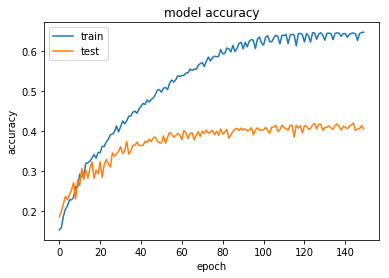
\includegraphics[width=\linewidth]{img/enc-dec-2.png}
    \caption{Resultados de Acurácia por Época}
  \end{subfigure}
  \begin{subfigure}[b]{0.45\linewidth}
    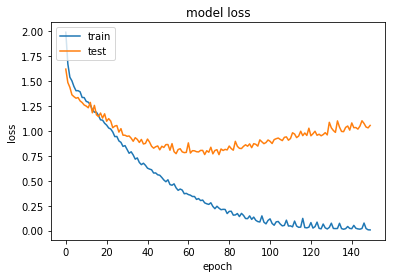
\includegraphics[width=\linewidth]{img/enc-dec-2-loss.png}
    \caption{Resultados de Custo por Época}
  \end{subfigure}
  \caption{Gráficos dos Resultados do Modelo}
  \label{fig:plots2}
\end{figure}

\begin{table}[H]
\centering
\begin{tabular}{llllll}
\textbf{Best Epoch Score} & \textbf{Val\_Acc} & \textbf{Vall\_Loss} & \textbf{Loss} & \textbf{Acc} & \textbf{Time} \\
145 & 0.419 & 1.048 & 0.014 & 0.644 & 4 min
\end{tabular}
\caption{Scores do Modelo Encoder-Decoder 2}
\label{tab:res-enc-dec-2}
\end{table}

\subsection{Modelo Encoder-Decoder 3}
 
\subsubsection{Corpus}

O corpus utilizado para o treinamento das redes \textbf{Encoder-Decoder 3}, \textbf{Encoder-Decoder 4} e \textbf{Encoder-Decoder 5}  foi baseado na lista de verbos disponíveis no site \url{https://www.conjugacao.com.br/verbos-populares/}.\\

As informações contidas nessa página diferem-se das páginas apresentadas na Seção \ref{sec:corpus-ffd} no sentido de que, em primeiro lugar, não há qualquer divisão entre verbos regulares ou irregulares (o que dificulta a segmentação manual dos verbos em diferentes famílias); apesar disso, ganha-se ao aumentar em quase cem vezes o tamanho da base de treino. 

Assim como na Seção \ref{sec:corpus-ffd}, foi realizada uma etapa de extração dos verbos e suas respectivas conjugações para um banco de dados local. Em seguida, os verbos foram mantidos em notação ortográfica como um exercício de prova de conceito. O objetivo dos testes que se seguem é avaliar o potencial preditivo quando se pode contar com uma base de treinamento consideravelmente maior. Perde-se pela considerável redução de resolução com relação ao reconhecimento de padrões fonológicos, fato que será discutido na Seção \ref{sec:disc}

\subsubsection{Hiperparâmetros} 

\begin{table}[H]
\centering
\begin{tabular}{ll}
Numero de Amostras Treinamento: & 2000 \\
Numero de Amostras Teste: & 100 \\
Numero de tokens unicos do Input: & 26 \\
Numero de tokens unicos do Output: & 32 \\
Comprimento maximo da sequencia para inputs: & 15 \\
Comprimento maximo da sequencia para outputs: & 16 \\
Loss: & categorical\_crossentropy \\
Optimizer & rmsprop \\
Activation & softmax \\
Epochs & 100 \\
Batch Size & 64
\end{tabular}
\caption{Tabela Resumo Estrutural do Modelo Encoder-Decoder 3}
\label{tab:res3}
\end{table}

\subsubsection{Resultados}
%falar q eu adicionei dropout e explicar oq é isso

\begin{figure}[H]
  \centering
  \begin{subfigure}[b]{0.45\linewidth}
    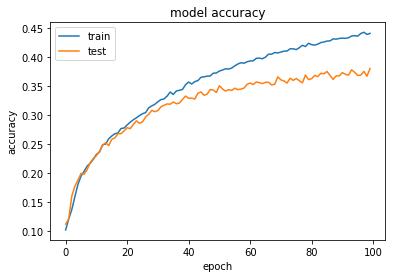
\includegraphics[width=\linewidth]{img/enc-dec-3.png}
    \caption{Resultados de Acurácia por Época}
  \end{subfigure}
  \begin{subfigure}[b]{0.45\linewidth}
    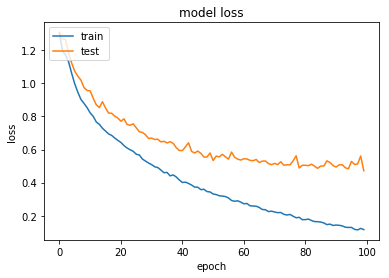
\includegraphics[width=\linewidth]{img/enc-dec-3-loss.png}
    \caption{Resultados de Custo por Época}
  \end{subfigure}
  \caption{Gráficos dos Resultados do Modelo}
  \label{fig:plots3}
\end{figure}

\begin{table}[H]
\centering
\begin{tabular}{llllll}
\textbf{Best Epoch Score} & \textbf{Val\_Acc} & \textbf{Vall\_Loss} & \textbf{Loss} & \textbf{Acc} & \textbf{Time} \\
100 & 0.380 & 0.471 & 0.115 & 0.440 & 11 min
\end{tabular}
\caption{Scores do Modelo Encoder-Decoder 3}
\label{tab:res-enc-dec-3}
\end{table}

\subsection{Modelo Encoder-Decoder 4}
%Falar que eu quis mudar a funcao de ativacao pra ver oq acontecia e o otimizador tb (deve ter tido uma razao pra eu ter feito isso, deve ta no deep learning la)

\subsubsection{Hiperparâmetros} 

\begin{table}[H]
\centering
\begin{tabular}{ll}
Numero de Amostras Treinamento: & 2000 \\
Numero de Amostras Teste: & 100 \\
Numero de tokens unicos do Input: & 26 \\
Numero de tokens unicos do Output: & 29 \\
Comprimento maximo da sequencia para inputs: & 15 \\
Comprimento maximo da sequencia para outputs: & 16 \\
Loss: & categorical\_crossentropy \\
Optimizer & adam \\
Activation & relu \\
Epochs & 100 \\
Batch Size & 64
\end{tabular}
\caption{Tabela Resumo Estrutural do Modelo Encoder-Decoder 4}
\label{tab:res4}
\end{table}

\subsubsection{Resultados}
%falar q eu adicionei dropout e explicar oq é isso

\begin{figure}[H]
  \centering
  \begin{subfigure}[b]{0.45\linewidth}
    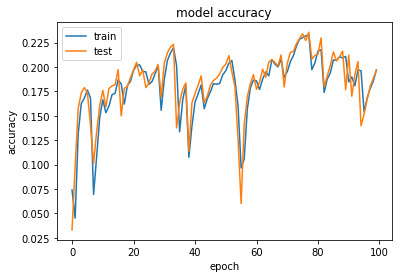
\includegraphics[width=\linewidth]{img/enc-dec-4.png}
    \caption{Resultados de Acurácia por Época}
  \end{subfigure}
  \begin{subfigure}[b]{0.45\linewidth}
    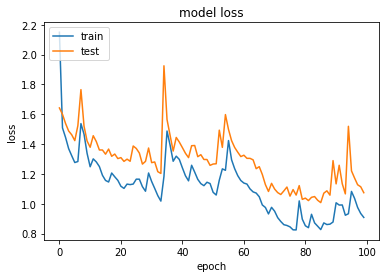
\includegraphics[width=\linewidth]{img/enc-dec-4-loss.png}
    \caption{Resultados de Custo por Época}
  \end{subfigure}
  \caption{Gráficos dos Resultados do Modelo}
  \label{fig:plots4}
\end{figure}

\begin{table}[H]
\centering
\begin{tabular}{llllll}
\textbf{Best Epoch Score} & \textbf{Val\_Acc} & \textbf{Vall\_Loss} & \textbf{Loss} & \textbf{Acc} & \textbf{Time} \\
86 & 0.210 & 1.00 & 0.820 & 0.207 & 10 min
\end{tabular}
\caption{Scores do Modelo Encoder-Decoder 4}
\label{tab:res-enc-dec-4}
\end{table}

 
 \subsection{Modelo Encoder-Decoder 5}
%Falar que eu quis aumentar mais ainda a amostra

\subsubsection{Hiperparâmetros} 

\begin{table}[H]
\centering
\begin{tabular}{ll}
Numero de Amostras Treinamento: & 3000 \\
Numero de Amostras Teste: & 100 \\
Numero de tokens unicos do Input: & 26 \\
Numero de tokens unicos do Output: & 32 \\
Comprimento maximo da sequencia para inputs: & 15 \\
Comprimento maximo da sequencia para outputs: & 16 \\
Loss: & categorical\_crossentropy \\
Optimizer & rmsprop \\
Activation & softmax \\
Epochs & 100 \\
Batch Size & 64
\end{tabular}
\caption{Tabela Resumo Estrutural do Modelo Encoder-Decoder 5}
\label{tab:res5}
\end{table}

\subsubsection{Resultados}
%falar q eu ainda nao adicionei o dropout mas pode ser legal adicionar

\begin{figure}[H]
  \centering
  \begin{subfigure}[b]{0.45\linewidth}
    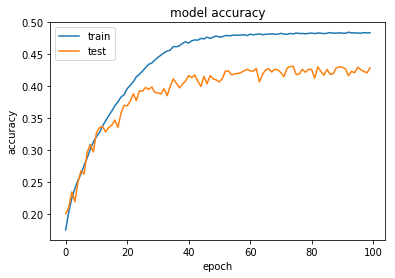
\includegraphics[width=\linewidth]{img/enc-dec-5.png}
    \caption{Resultados de Acurácia por Época}
  \end{subfigure}
  \begin{subfigure}[b]{0.45\linewidth}
    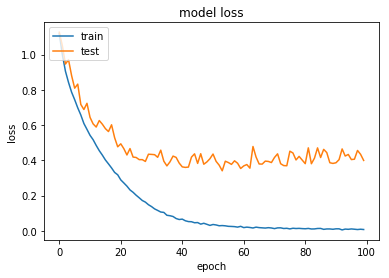
\includegraphics[width=\linewidth]{img/enc-dec-5-loss.png}
    \caption{Resultados de Custo por Época}
  \end{subfigure}
  \caption{Gráficos dos Resultados do Modelo}
  \label{fig:plots5}
\end{figure}

\begin{table}[H]
\centering
\begin{tabular}{llllll}
\textbf{Best Epoch Score} & \textbf{Val\_Acc} & \textbf{Vall\_Loss} & \textbf{Loss} & \textbf{Acc} & \textbf{Time} \\
54 & 0.423 & 0.340 & 0.030 & 0.4789 & 15 min
\end{tabular}
\caption{Scores do Modelo Encoder-Decoder 5}
\label{tab:res-enc-dec-5}
\end{table}

\section{Discussão}
\label{sec:disc}

Na Tabela \ref{tab:resultadosfdd} observa-se que aparentemente não há qualquer relação entre a proporção de verbos irregulares na base de treino e a acurácia do modelo. A acurácia foi cálculada a partir de uma base de teste em que considera-se um acerto apenas quando a sequência predita corresponde exatamente à sequência esperada. Apesar da variação percentual ser grande, os modelos podem ser considerados similares pois a base de teste era de apenas 21 verbos e uma predição incorreta de uma única conjugação significa uma perda de 4.76\% na acurácia. Tal variação pode ter ocorrido por motivos aleatórios, uma vez que o processo em questão não é determinístico e envolve diversos procedimentos algébricos que podem refletir nos valores dos pesos. Com relação à métrica \textit{Loss}, observa-se que há relação entre o aumento da proporção de verbos irregulares e a sua respectiva diminuição. Essa métrica foi cálculada pelo próprio modelo durante o treinamento. Isso indica que a maior presença destes verbos ajudou, ainda que minimamente, na redução do erro quadrático médio. Essa redução não se converteu em ganho considerável de acurácia, por possivelmente duas razões: não houve aumento no número de exemplos distintos de verbos irregulares, somente no número de vezes que um mesmo verbo passou pelo treinamento. Isto pode provocado um \textit{overfitting} nos dados; ou, a função de decodificação proposta pode ter sido insuficiente para distinguir suficientemente fonemas próximos, como observado nos resultados do Apêndice. %linhas tal tal e tal

Os modelos Encoder-Decoder foram considerados principalmente pela independência de funções de decodificação para sequências. O cálculo recursivo a nível de caracter utilizando as LSTM's elimina o problema apontado na Seção \ref{sec:dec}. No entanto, como verificado nas figuras \ref{fig:plots1} e \ref{fig:plots2}, a grande distância entre a acurácia de treino e validação ainda indica \textit{overfitting}. Por essa razão, viu-se necessário o aumento da base de treino e o acréscimo de uma camada de \textit{Dropout}\footnote{Dropout é uma técnica de regularização que inativa aleatóriamente algumas unidades durante o treinamento. %ref
} = 0.25. Os resultados do modelo \textbf{Encoder-Decoder 3} (Fig. \ref{fig:plots3}) treinados em 2000 verbos distintos indicam redução notável na diferença entre os resultados obtidos para teste e validação. Ainda que tais resultados sejam inferiores aos obtidos pelos modelos \textbf{Encoder-Decoder 1} e \textbf{Encoder-Decoder 2}, deve-se lembrar que houve redução de resolução e acréscimo de features, uma vez que a base de treino é composta por verbos em notação ortográfica e não fonética. 

O modelo \textbf{Encoder-Decoder 4} foi desenvolvido com o objetivo de se testar uma diferente função de ativação. De acordo com %deeplearning tal tal
, sugere-se a utilização do otimizador "Adam" em conjunto com a função de ativação "RELU". Os resultados exibidos na Figura \ref{fig:plots4} demonstram um aprendizado completamente instável e fraco. 

Por último, o modelo \textbf{Encoder-Decoder 5} foi treinado em uma base de 3000 verbos distintos sem camada de Dropout e conseguiu o melhor resultado de acurácia (0.423) para o grupo de validação entre os modelos dessa mesma arquitetura. Com relação à outra arquitetura (FDD), a comparação torna-se de certa forma injusta pois, em primeiro lugar, a rede FDD é incapaz de gerar sequências maiores que quatro caracteres como discutido na Seção \ref{sec:dec}. Em segundo lugar, as bases de teste aplicadas são distintas: A base de teste da FDD é 30 vezes menor e é mais controlada com relação às irregularidades presentes.\\

Em resumo, os resultados obtidos até agora indicam que: 

\begin{enumerate}
\item Aumentar a base de treino parece aprimorar o aprendizado de forma razoável;
\item Aumentar o grau de resolução para transcrição fonética nessa mesma base pode aprimorar o aprendizado ainda mais (como observado nos resultados do modelo Encoder-Decoder 2);
\item O acréscimo da camada de Dropout surtiu um efeito muito interessante e a combinação com os demais itens apontados pode contribuir ainda mais para o aprimoramento do modelo.
\end{enumerate}

%\textit{1. Aumentar a base de treino parece aprimorar o treinamento de forma razoável}; \textit{2. Aumentar o grau de resolução para transcrição fonética nessa mesma base pode aprimorar o treinamento ainda mais (como observado nos resultados do modelo Encoder-Decoder 2)}; \textit{3. O acréscimo da camada de Dropout surtiu um efeito muito interessante e a combinação com os demais itens apontados pode contribuir ainda mais para o aprimoramento do modelo}.
